\documentclass[../../main.tex]{subfiles}

\begin{document}
\label{sec:abbildungen_explizite_schreibweise}
Wie im letzten Abschnitt erklärt wurde, formen Funktionen Elemente einer Definitionsmenge in Elemente einer Zielmenge um. Dabei folgen sie einer gewissen Zuordnungsvorschrift. Sie beschreibt, welches Element der Definitionsmenge welches Bild erhält.

Die Zuordnungsvorschrift kann auf verschiedenen Wegen beschrieben werden. Im letzten Abschnitt hast du die Zuordnungsvorschrift aufgeschrieben, indem du für jedes Element der Definitionsmenge explizit aufgeschrieben hast, welches Bild es erhält. Wie man das außerdem noch machen kann, lernst du in diesem Abschnitt.

\subsection{Explizite Schreibweise}

Du kannst eine Zuordnungsvorschrift durch das Hintereinanderschreiben von Zuordnungsregeln auflisten. Im letzten Abschnitt waren alle Definitionsmengen, die du gesehen hast, sehr klein. Sie enthielten allesamt nur sehr wenige Elemente. Deshalb war es möglich, einzeln zu jedem Element aus der Definitionsmenge aufzuschreiben, welchem Bild es zugeordnet wird.

\begin{example}{}
    \parpic[r]{
        \begin{tikzpicture}[scale=.6]
            \draw[grayset] (-1.5,0) ellipse (2.2cm and 2.7cm);
            \draw[grayset] (3.5,0) ellipse (1.9cm and 2.7cm);
            %
            \node[label={[blue!50!black]left:Mo}, blue!50!black] (x1) at (-1,1.6) {$\bullet$};
            \node[label={[blue!50!black]left:Di}, blue!50!black] (x2) at (-1,0.7) {$\bullet$};
            \node[label={[blue!50!black]left:Mi}, blue!50!black] (x3) at (-1,-0.2) {$\bullet$};
            \node[label={[blue!50!black]left:Do}, blue!50!black] (x4) at (-1,-1.1) {$\bullet$};
            \node[label={[blue!50!black]left:Fr}, blue!50!black] (x5) at (-1,-2) {$\bullet$};
            %
            \node[orange] (y1) at (3.5,0) {
\includegraphics[width=1cm]{images/weather.png}};
            %
            \draw[->] (x1) -- (2.8,0.2);
            \draw[->] (x2) -- (2.8,-1.4);
            \draw[->] (x3) to[bend right] (2.8,0.1);
            \draw[->] (x4) -- (2.8,1.2);
            \draw[->] (x5) to[bend right] (2.8,-1.5);
        \end{tikzpicture}
    }
    Kurz vor oder nach den Nachrichten in Fernsehen oder Radio gibt es einen Wetterbericht, damit man sich auf die nächsten Tage einstellen kann und keine Radtour bei heftigem Gewitter plant.
    
    \picskip{2}
    Oftmals gibt es eine Vorschau über mehrere Tage mit dem wahrscheinlichsten Wetter für jeden Tag. Nachdem du eine solche Vorschau gesehen hast, weißt du beispielsweise, dass es am nächsten Montag Schauer geben wird, während es am Donnerstag trocken bleibt. Die Zuordnung von Wochentagen zum vorhergesagten Wetter, die du dann kennst, ist aus mathematischer Sicht eine Funktion.
    
    An welchem Wochentag es welches Wetter gibt, kann durch eine Funktion von den Wochentagen auf das entsprechende Wetter dargestellt werden, die wir \textsc{Vorhersage} nennen wollen. Wir arbeiten also mit den Mengen \[\textsc{Wochentag}\coloneqq\{\text{Montag},\text{Dienstag},\text{Mittwoch},\text{Donnerstag},\text{Freitag}\}\] und \[\textsc{Wetter}\coloneqq\{\text{Trocken},\text{Schauer},\text{Gewitter}\}.\]
    Die Zuordnungsvorschrift (zu sehen im Bild) lässt sich dann durch Auflisten der Vorhersagen aufschreiben und sieht so aus:
    \begin{align*}
        \textsc{Vorhersage}(\text{Montag})&=\text{Schauer},\\ \textsc{Vorhersage}(\text{Dienstag})&=\text{Gewitter},\\ \textsc{Vorhersage}(\text{Mittwoch})&=\text{Schauer},\\ \textsc{Vorhersage}(\text{Donnerstag})&=\text{Trocken},\\ \textsc{Vorhersage}(\text{Freitag})&=\text{Gewitter}.
    \end{align*}
    Natürlich würde kein Nachrichtensender der Welt seinen Wetterbericht in dieser Form darstellen. Du wirst gleich sehen, welche übersichtlicheren Möglichkeiten es gibt.
\end{example}

Die Zuordnungsvorschrift ist auf diese Weise eine (möglicherweise sehr lange) Liste von einzelnen Regeln -- je eine Regel pro möglichem Argument (also Element der Definitionsmenge).
Mithilfe der mathematischen Notation aus dem letzten Abschnitt schreibst du alle Paare aus Urbild und Bild entweder als \mbox{$\text{Urbild}\mapsto\text{Bild}$} oder, wenn du eine Funktion mit dem Namen $f$ beschreibst, als \mbox{$f(\text{Urbild})=\text{Bild}$}. Weil du zu jedem Argument explizit aufschreibst, welches Bild es bekommt, kann man dies auch eine \emph{explizite} Zuordnungsvorschrift nennen.

Der größte Nachteil dieser sehr einfachen Möglichkeit ist, dass eine solche Liste sehr unübersichtlich wird, wenn du mit großen Definitionsmengen arbeitest. Darüber hinaus kennst du bereits unendliche Mengen (wie beispielsweise die Menge \Natural{} der natürlichen Zahlen). Für unendliche Definitionsmengen ist es sogar unmöglich, allen Elementen explizit ein Bild zuzuordnen.

\subsection{Wertetabellen\index{Wertetabelle}}
\label{sec:abbildungen_wertetabellen}

Du hast bereits die explizite Schreibweise für das Notieren von Zuordnungsvorschriften kennengelernt. Außerdem kennst du nun den Nachteil, dass sich mit der expliziten Schreibweise große Definitionsmengen sehr schlecht oder sogar überhaupt nicht vertragen. In diesem Abschnitt siehst du eine andere Darstellungsart, in der du Zuordnungsvorschriften oft vorfinden wirst.

\begin{example}{}
    \parpic[r]{
        \begin{tabular}{cc}\toprule
            Tag & Vorhersage\\\midrule
            Montag & Schauer\\
            Dienstag & Gewitter\\
            Mittwoch & Schauer\\
            Donnerstag & Trocken\\
            Freitag & Gewitter\\\bottomrule
        \end{tabular}
    }
    
    Die Wettervorhersage für die kommende Woche wird sicherlich nirgends wie im letzten Beispiel mathematisch notiert sein. Viel häufiger wirst du eine Darstellung wie in der rechts abgebildeten Tabelle finden. Dort ist ebenfalls klar zu erkennen, dass es zum Beispiel am Freitag gewittern wird.
    
    In jeder Zeile der Tabelle findest du einen Wochentag und -- daneben -- das Wetter, das für diesen Wochentag vorhergesagt ist.
\end{example}

Wenn es darum geht, Daten übersichtlich und strukturiert darzustellen, kommen häufig Tabellen zum Einsatz. Auf sehr einfache Weise können Tabellen auch Zuordnungsvorschriften darstellen.

In \textbf{Wertetabellen}, die eine Funktion beschreiben, findest du normalerweise zwei Spalten: Die linke Spalte enthält alle Urbilder, also alle Elemente der Definitionsmenge der Funktion. In der rechten Spalte steht das Element der Zielmenge, das die Funktion ihm zuordnet. Die gleichen Urbild-Bild-Paare, die sonst durch $\text{Urbild}\mapsto\text{Bild}$ notiert wurden, stehen jetzt also einfach nebeneinander in derselben Zeile.

\parpic[r]{
    \begin{tabular}{cc}\toprule
        $x$ & $f(x)$\\\midrule
        0 & 1\\
        1 & 2\\
        \dots & \dots\\\bottomrule
    \end{tabular}
}

Allgemein sieht die Wertetabelle für eine Funktion namens $f$ ungefähr so aus wie rechts abgebildet. Zu lesen ist das folgendermaßen: Auf der linken Seite stehen alle Werte (hier mit der Variablen $x$ bezeichnet), die sich potentiell mit der Funktion auf andere Dinge abbilden lassen. Schaust du in die linke Spalte und findest dort beispielsweise die $0$, dann steht rechts davon das Bild der $0$, also $f(0)$. 

In der Zeile mit der $0$ stehen die Werte $0$ und $f(0)$ nebeneinander. Dass die $0$ und die $1$ in der abgebildeten Tabelle in derselben Zeile stehen, bedeutet also, dass $f(0)=1$ gilt. Jede Zeile einer Wertetabelle kannst du deshalb so lesen, dass die Funktion dem linken Wert den rechten Wert zuordnet.

Weil Tabellen einfacher zu verwenden sind als mathematische Vorschriften, wirst du häufig sehen, dass Funktionen durch Tabellen beschrieben werden statt -- wie im letzten Abschnitt -- formal mathematisch. Ergebnisse von Versuchen, Informationen in Büchern oder im Internet und viele weitere Zusammenhänge sind in Tabellen organisiert.

Letztendlich schreibt man mit Tabellen immer noch für jedes einzelne Element der Definitionsmenge auf, welches Bild es erhält. In jeder solchen Wertetabelle steckt also eine explizite Zuordnungsvorschrift (auch wenn sie nicht direkt aufgeschrieben ist -- man könnte aus der Tabelle eine explizite Zuordnungsvorschrift produzieren). Wichtig ist, dass du dir über diesen Zusammenhang bewusst bist und mit beiden Darstellungen umgehen kannst. Insbesondere solltest du also im Hinterkopf haben, wie du aus einer Tabelle herauslesen kannst, welche Funktion sie beschreibt.

Im nächsten Beispiel siehst du noch einmal Schritt für Schritt, wie du mit einer gegebenen Wertetabelle herausfindest, welche Funktion man mit ihr beschreibt.

\begin{example}{}
    \parpic[r]{
        \begin{tabular}{cc}\toprule
            Land & Hauptstadt \\\midrule
            Italien & Rom\\
            Spanien & Madrid\\
            Belgien & Brüssel\\
            Norwegen & Oslo\\
            Frankreich & Paris\\
            Finnland & Helsinki\\
            Dänemark & Kopenhagen\\\bottomrule
        \end{tabular}
    }
    
    Auf der rechten Seite siehst du eine Tabelle von europäischen Ländern mit ihren Hauptstädten. Als erstes solltest du versuchen, als Satz formulieren, was die Tabelle aussagt, etwa \enquote{Die Tabelle ordnet europäischen Ländern ihre Hauptstädte zu.} Versuche am besten, den Satz so umzuordnen, dass er \enquote{ordnet zu} enthält.
    
    \picskip{3}
    Wenn du das machst, siehst du bereits die Definitions- und Zielmenge in deinem Satz. Mit genau solchen Sätzen haben wir nämlich auch schon mathematische Funktionen beschrieben.
    
    Nachdem du verstanden hast, welche Funktion in der Tabelle versteckt ist, kannst du sie mit der expliziten mathematischen Schreibweise darstellen. Überlege dir dafür zunächst einen Namen für die Funktion -- in diesem Fall ist \textsc{Hauptstadt} eine naheliegende Wahl. Anschließend lässt sich die Definitionsmenge als die Menge aller Einträge der linke Spalte beschreiben, also
    \[\textsc{Länder}\coloneqq\{\text{Italien},\text{Spanien},\text{Belgien},\text{Norwegen},\text{Frankreich},\text{Finnland},\text{Dänemark}\}.\]
    
    Auf die gleiche Weise enthält die Zielmenge alle Einträge der rechten Spalte:
    
    \[\textsc{Städte}\coloneqq\{\text{Rom},\text{Madrid},\text{Brüssel},\text{Oslo},\text{Paris},\text{Helsinki},\text{Kopenhagen}\}.\]
    
    \sloppy
    Die formal notierte Zuordnungsvorschrift besteht nun aus den Regeln \[\textsc{Hauptstadt}(\text{Italien})=\text{Rom}, \textsc{Hauptstadt}(\text{Spanien})=\text{Madrid}\] und so weiter -- für jede Zeile der Tabelle eine Regel. Damit ist die Funktion fertig beschrieben.
    \fussy
\end{example}

In diesem Beispiel hat die Funktion einen Namen bekommen, der sich aus dem Sachzusammenhang ergeben hat. Fällt dir kein solcher Name ein, verwende einfach $f, g$ oder $h$. Dies sind die Buchstaben, mit denen standardmäßig Funktionen beschrieben werden, denen sich nicht so einfach ein Name wie im letzten Beispiel zuordnen lässt. Wenn in der Tabelle zum Beispiel nur Zahlen stehen, ist es sinnvoll, auf solche Namen auszuweichen.

\begin{example}{}
    \parpic[r]{
        \begin{tabular}{cc}\toprule
            $x$ & $y$ \\\midrule
            $1$ & $2$\\
            $2$ & $3$\\
            $3$ & $5$\\
            $4$ & $7$\\
            $5$ & $11$\\\bottomrule
        \end{tabular}
    }
    
    Die abgebildete Tabelle lässt sich als Beschreibung einer Funktion interpretieren. Leider lässt nicht sofort durch einen Satz beschreiben, was die Funktion tut. Trotzdem kann man wie vorher vorgehen und als Definitionsmenge die Einträge der linken Spalte wählen.
    
    \picskip{4}
    Da die linke Spalte mit $x$ überschrieben ist, nennen wir die Definitionsmenge $X$. Dann ist $X=\{1,2,3,4,5\}$. Die Zielmenge besteht aus allen Zahlen, die in der rechten Spalte stehen, also $Y=\{2,3,5,7,11\}$. Weil nicht klar ist, was die Funktion genau tut, erhält sie einfach den Namen $f$.
    
    Folglich ist $f$ eine Funktion von $X$ nach $Y$, geschrieben also $f\colon X\rightarrow Y$. Dabei gilt $f(1)=2, f(2)=3, f(3)=5, f(4)=7$ und $f(5)=11$ (wieder sind das jeweils die Werte, die in den Zeilen nebeneinander stehen).
\end{example}

\subsection{Berechnungsvorschriften\index{Berechnungsvorschrift}}
\label{sec:abbildungen_berechnungsvorschriften}

Mit der expliziten Schreibweise für Zuordnungsvorschriften, die du in den letzten Abschnitten kennengelernt hast, lassen sich alle möglichen Funktionen beschreiben, bei denen die Definitionsmenge klein genug ist, damit das Notieren der Zuordnungsvorschrift nicht in stundenlangem Schreibaufwand ausartet. Stelle dir zum Beispiel vor, du müsstest eine Zuordnungsvorschrift explizit für eine Definitionsmenge, die 100 Elemente enthält, aufschreiben. Abgesehen davon, dass dies extrem viel Aufwand bedeutet, ist das Ergebnis außerdem nicht hilfreich, weil es viel zu lang ist.

Aus diesem Grund lernst du nun, Funktionen so zu analysieren, dass du nicht für jedes Element der Definitionsmenge einzeln das Bild aufschreiben musst, sondern nach einer \emph{Regel} suchst, die beschreibt, was die Funktion mit ihren Argumenten macht, ohne für jedes Element einzeln aufzuschreiben, welches Ergebnis genau herauskommt. 

Es gibt -- vor allem im Alltag -- viele Funktionen, die man tatsächlich nur dadurch beschreiben kann, welches Urbild welches Bild hat. Dazu gehören zum Beispiel Vokabeln, Hauptstädte oder Wettervorhersagen.

Aus mathematischer Sicht interessant sind aber vor allem Funktionen, bei denen es genau so eine Regel gibt.

\begin{example}[ex:buchstabenanzahl]{}
    \parpic[r]{
        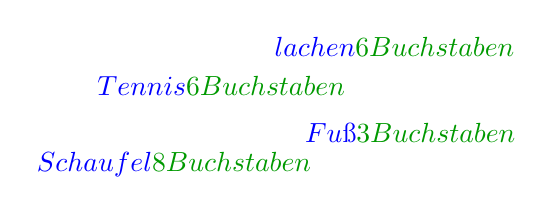
\begin{tikzpicture}
            \node[blue] at (0,0) {$\colorbrace{\text{Schaufel}}{\textcolor{green!60!black}{\text{8 Buchstaben}}}$};
            \node[blue] at (0.6,1) {$\colorbrace{\text{Tennis}}{\textcolor{green!60!black}{\text{6 Buchstaben}}}$};
            \node[blue] at (3,0.4) {$\colorbrace{\text{Fuß}}{\textcolor{green!60!black}{\text{3 Buchstaben}}}$};
            \node[blue] at (2.8,1.5) {$\colorbrace{\text{lachen}}{\textcolor{green!60!black}{\text{6 Buchstaben}}}$};
        \end{tikzpicture}
    }

    Jedes Wort in deutscher Sprache besteht aus einer bestimmten Anzahl von Buchstaben. Eine Funktion, die jedem Wort die Anzahl seiner Buchstaben zuordnet, folgt der klaren Regel, die Buchstaben zu zählen.
    
    \picskip{1}
    Die Zuordnungsvorschrift kann deshalb angegeben werden, indem man sagt: \emph{Egal welches Wort du abbilden musst, zähle seine Buchstaben und schreibe das Ergebnis auf.} 
    
    Wenn man nun herausfinden möchte, welches Bild die Funktion $\textsc{Buchstabenanzahl}$ dem Wort \emph{Lampe} zuordnet, dann lässt sich die Antwort $5$ finden, obwohl vorher keine Liste mit Urbild-Bild-Paaren aufgeschrieben wurde.
\end{example}

Existiert eine klare Regel, mit der man aus einem beliebigen Element der Definitionsmenge sein Bild bestimmen kann, dann ist es auch ausreichend, diese Regel aufzuschreiben. Dadurch wird ebenfalls jede Zuordnung der Zuordnungsvorschrift festgelegt. Statt aus einer langen Liste den richtigen Wert herauszusuchen, ist es dann nötig, die Regel auf das Element, das man abbilden möchte, anzuwenden.

Um eine solche Regel aufzuschreiben, musst du eine Variable nutzen, mit der du das Element, das man gerade abbilden möchte, beschreibst. Meistens nutzt man dafür die Variablennamen $x$ oder $n$. Statt nun für alle Elemente der Definitionsmenge einzelne Regeln aufzuschreiben, reicht es, einmal wie folgt die Regel aufzuschreiben (hier soll die Zuordnungsvorschrift für eine Abbildung $f$ festgelegt werden): 
\[f(x)=\textit{Regel, mit der aus $x$ das Bild von $x$ berechnet werden kann}\]

\begin{example}{}
    Im letzten Beispiel kann die Regel, mit der die Funktion \textsc{Buchstabenanzahl} ihrem Argument ein Bild zuordnet, mit
    \[\textsc{Buchstabenanzahl}(x)=\text{Anzahl~der~Buchstaben~von~}x\]
    beschrieben werden.
\end{example}

Um mithilfe einer Berechnungsvorschrift für ein \emph{beliebiges} Argument von $f$ sein Bild zu berechnen, musst du schauen, was auf der rechten Seite vom Gleichheitszeichen steht, wenn du den konkreten Wert für $x$ einsetzt, den du in die Funktion einsetzen möchtest. Mit der Berechnungsvorschrift muss es möglich sein, die rechte Seite dann so auszuwerten, dass man direkt das Bild von $x$ erhält.

Das nächste Beispiel behandelt noch einmal die Funktion, die Farben mit gelb mischt und schlägt eine Berechnungsvorschrift vor, die man für diese Funktion verwenden kann. Anschließend siehst du ein Beispiel mit einer etwas mathematischeren Berechnungsvorschrift.

\begin{example}{}
    \parpic[r]{
        \begin{tikzpicture}[scale=.6]
    \fill[grayset] (-1.5,0) ellipse (2.4cm and 2cm);
    \fill[grayset] (4,0) ellipse (2.4cm and 2cm);
    %
    \node[label={[blue]left:blau}, blue] (x1) at (-1,0.7) {$\bullet$};
    \node[label={[red]left:rot}, red] (x2) at (-1,-0.2) {$\bullet$};
    \node[label={[yellow!70!black]left:gelb}, yellow!70!black] (x3) at (-1,-1.1) {$\bullet$};
    %
    \node[label={[green!70!black]right:grün}, green!70!black] (y1) at (3.5,0.7) {$\bullet$};
    \node[label={[orange]right:orange}, orange] (y2) at (3.5,-0.2) {$\bullet$};
    \node[label={[yellow!70!black]right:gelb}, yellow!70!black] (y3) at (3.5,-1.1) {$\bullet$};
    %
    \draw[->] (x1) to[bend left] (y1);
    \draw[->] (x2) -- (y2);
    \draw[->] (x3) to[bend right] (y3);
\end{tikzpicture}%Also used by abbildungen/02_formale_schreibweisen
    }
    
    Mischt man die drei Grundfarben mit gelb, erhält man eine Abbildung von einer Grundfarbe auf ihre jeweilige Mischfarbe mit gelb, zum Beispiel wird blau auf die Farbe grün abgebildet, weil dies die Farbe ist, die man erhält, wenn man blau und gelb mischt.
    
    \picskip{0}
    Es ist klar, welche Grundfarbe wie abgebildet wird, ohne dass dies explizit einzeln für jede Grundfarbe aufgeschrieben werden muss, weil die Regel, nach der man aus einer Farbe bestimmt, in welche andere Farbe sie übersetzt wird, feststeht. Mit anderen Worten: Schreibt man als Zuordnungsvorschrift
    \[\textsc{MitGelbMischen}(x)=\text{Farbe, die beim Mischen von } x \text{ mit gelb entsteht},\]
    dann ist trotzdem noch eindeutig klar, wie die Abbildung mit \textsc{MitGelbMischen} funktioniert.
\end{example}

\begin{example}{}
    \parpic[r]{
\includegraphics[width=.2\textwidth]{images/kuh.pdf}}

    \picskip{5}
    Ein Bauer verkauft frische Milch zu einem Preis von 2 Euro pro Liter. Wenn ein Kunde Milch kauft, hängt der Preis, den er zahlen muss, natürlich davon ab, \emph{wie viel} Milch er kauft. Mithilfe einer Funktion \[\textsc{Preis}\colon\Natural\rightarrow\Natural,\] die die Anzahl an Litern Milch, die gekauft werden, ihrem Preis in Euro zuordnet, kann für eine gegebene Menge Milch ermittelt werden, wie teuer sie ist. Wir lassen die Einheiten weg, damit wir mit Zahlen arbeiten können.
    
    Statt für jede Menge Milch einzeln aufzulisten, wie viel sie kostet (etwa \mbox{$\textsc{Preis}(1)=2$}, $\textsc{Preis}(2)=4$ usw.), ist es auch möglich, einfach den Preis für eine beliebige Menge Milch anzugeben. Dafür bezeichnen wir die Menge Milch, die gekauft wird, mit $m$ (in Litern). Egal, welche Zahl $m$ wir wählen: Es gilt immer, dass der Preis in Euro doppelt so groß wie $m$ ist, also \[\textsc{Preis}(m)=2\cdot m.\]
    Diese Regel genügt, um die Zuordnungsvorschrift vollständig festzulegen. Beispielsweise ist der Preis von 12 Litern Milch (in Euro) \mbox{$\textsc{Preis}(12)=2\cdot 12=24$}.
\end{example}

\begin{nutshell}{Arten von Zuordnungsvorschriften\index{Wertetabelle}\index{Berechnungsvorschrift}}
    Die Regel, nach der eine Funktion $f$ ihren Argumenten aus der Definitionsmenge Bilder zuordnet -- also die Zuordnungsvorschrift -- kann auf verschiedene Weisen aufgeschrieben werden:
    \begin{enumerate}[label=\textbf{(\arabic*)}]
        \item \textbf{mit der expliziten Schreibweise}\\
            \sloppy
            Zu jedem Element der Definitionsmenge schreibst du \emph{explizit} auf, welches Bildelement ihm zugeordnet wird. Dafür nutzt du die Schreibweise \mbox{$f(\text{Argument})=\text{Bild}$} und listest für jedes Element der Definitionsmenge eine solche Regel auf.
        
            \fussy
        \item \textbf{mit einer Wertetabelle}\\
            Du zeichnest eine Tabelle mit zwei Spalten. In der linken Spalte trägst du alle Elemente der Definitionsmenge ein. In der rechten Spalte schreibst du neben jedes Element der Definitionsmenge das Bild, in das es von der Funktion übersetzt wird.
        
        \item \textbf{mit einer Berechnungsvorschrift}\\
            Hier gibst du an, wie aus einem \emph{beliebigen} Element $x$ der Definitionsmenge bestimmt werden kann, welches Bild es erhält. Dafür schreibst du
            \[f(x)=\textit{Regel, mit der aus $x$ das Bild von $x$ berechnet werden kann}.\]
    \end{enumerate}
\end{nutshell}

\end{document}